\chapter{Struktura programového řešení}
Struktura celého programového řešení je znázorněna na obrázku \ref{fig:speedy}. Celý projekt funguje následovně. Jednotlivé mikrokontroléry, resp. koncentrátory snímají potřebné veličiny, nebo čekají na impulz od uživatele sítě popř. serveru. Mohou tedy aktivně odesílat snímané informace, nebo reagovat na přijatý signál ze serveru. Tyto koncentrátory komunikují s real-time serverem pomocí protokolů TCP nebo UDP podle toho, jaký druh komunikace je pro daný účel potřeba. Server veškeré přijaté hodnoty ukládá do databáze a zároveň při každé příchozí akci prohlásí zařízení za aktivní. Udržuje tak neustále jeho status. Kromě toho, že server do databáze hodnoty ukládá, tak si také drží jednotlivé relace mezi koncentrátory resp. koncovými členy a odesílá data zpět. Tvoří tak jednotlivá propojení koncentrátorů, která je možné dynamicky měnit. Toto je asi největší výhoda tohoto řešení. Zároveň mají koncentrátory možnost zapisovat do databáze přímo. Je to dáno tím, že i se serverem komunikují v RESP formátu. Tato funkce není využívána, protože by bylo zapotřebí zapsat tvar databáze do každého koncentrátoru, což by bylo velmi omezující pro další rozšiřitelnost projektu. Nicméně tato možnost zde je a je možné ji využít pro rychlejší ukládání do databáze.

Na serveru dále běží webový server, který poskytuje webovou stránku, kde je možné celou síť ovládat. Každý uživatel sítě se pak může připojit pomocí svého zařízení (mobilní telefon, tablet, notebook, počítač, atd.) a síť ovládat. Je zřejmé, že je nutné umožnit pohodlné ovládání sítě, zároveň však musí být zamezena možnost změny konfigurace neautorizované osobě. Toto omezení je možné udělat na straně webové aplikace pomocí řízení uživatelských práv. Fakticky se jedná o změny relací v síti a o změnu parametrů jednotlivých koncových členů. Server se pak postará o distribuci dat v síti podle zvolené konfigurace.

\begin{figure}[H]
    \centering
	\makebox[\textwidth]{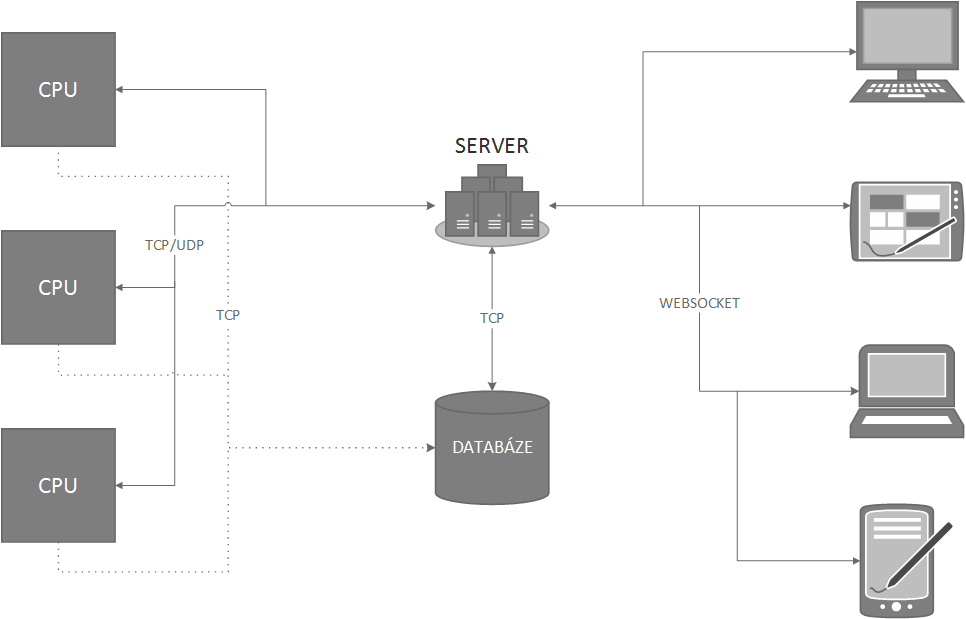
\includegraphics[width=\textwidth]{img/speedy.png}}
	\caption{Struktura programového řešení}
	\label{fig:speedy}
\end{figure}

\section{Koncentrátory}
Systémový firmware pro koncentrátory \index{Mikrokontrolér} je napsán v programovacím jazyce C s využitím oficiálních Cube knihoven od STMicroelectronics. Jsou tady napsány nízkoúrovňově, ale se zachováním přijatelného programového pro\-stře\-dí. Koncentrátor má několik základních funkcí. Předně je jeho úkolem připojit se na pevně stanovenou IP adresu v síti. Ta je momentálně stanovena na \texttt{192.168.0.20:50000}. Koncentrátor se pak periodicky s frekvencí 1 Hz o\-hla\-šu\-je přes TCP serveru. Tato frekvence je zvolena libovolně s ohledem na rozumné vytížení sítě těmito jinak zbytečnými informačními pakety. Síť se tak zbytečně nevytěžuje a zároveň dochází k rychlému zaregistrování výpadku koncentrátoru. 1 Hz je navíc nejhorší případ, protože jakákoliv příchozí informace se zároveň považuje za ohlášení.

Struktura programu z pohledu adresářové struktury je následující. Zobrazeny jsou pouze důležité části programu:

\begin{figure}[H]
\dirtree{%
.1 concentrator. 
.2 Drivers. 
.3 BSP\DTcomment{knihovny pro konkrétní hardware}. 
.3 CMSIS\DTcomment{nízkoúrovňové definice}. 
.3 STM32F4xx\_HAL\_Driver\DTcomment{definice periferií}. 
.2 Inc\DTcomment{hlavičkové soubory}. 
.2 MDK-ARM\DTcomment{konfigurace projektu pro Keil}. 
.2 Middlewares\DTcomment{knihovny třetích stran (LwIP)}. 
.2 Src\DTcomment{zdrojové kódy aplikace}. 
.3 app\_ethernet.c\DTcomment{pomocný soubor pro práci s Ethernetem}. 
.3 ethernetif.c\DTcomment{hlavní soubor pro práci s Ethernetem}. 
.3 main.c\DTcomment{hlavní soubor aplikace}. 
.3 stm32f4xx\_hal\_msp.c\DTcomment{konfigurace periferií}. 
.3 smt32f4xx\_it.c\DTcomment{obsluha přerušení}. 
.3 tcp.c\DTcomment{soubor starající se o TCP komunikaci}. 
.3 udp.c\DTcomment{soubor starající se o UDP komunikaci}. 
.3 .... 
.2 Utilities\DTcomment{doplňkové knihovny}. 
}
\end{figure}

Hlavní část této práce se nachází v \texttt{Src} složce, zejména se pak jedná o soubory \texttt{main.c}, což je soubor obsahující hlavní program. Tento program využívá funkce z dalších souborů, jmenovitě pak například \texttt{tcp.c} a \texttt{udp.c}, které se již podle názvu starají o TCP resp. UDP spojení se serverem. Následuje zjednodušený popis hlavního programu včetně několika ukázek kódu.

Nejdůležitější funkcí v každém podobném programu je funkce \texttt{main(void)}. Jedná se totiž o funkci, která je zavolána po spuštění programu. Ta prvně volá funkci pro inicializaci HAL knihovny \texttt{HAL\_Init(void)} \cite{hal}. Následně je volána funkce pro nastavení systémových hodin \texttt{SystemClock\_Config(void)}, konfigurace BSP (\texttt{BSP\_Config(void)}), inicializace LwIP \index{LwIP} (\texttt{lwip\_init(void)}), konfigurace síťového rozhraní (\texttt{Netif\_Config(void)}), nastavení časovačů pomocí \texttt{TIM\_Config(void)} a nastavení ADC převodníku (\texttt{ADC\_Config(void)}). Toto nastavení zároveň všechny potřebné procesy startuje. Vždy když dojde k nějaké akci, jako je například stisk tlačítka, zavolá se tzv. callback (například \texttt{HAL\_GPIO\_EXTI\_Callback}), který je umístěn v souboru \texttt{main.c}. Zde se provedou další potřebné úkoly na základě této spouštěcí akce. Tím pádem není nutné mít veškerou logiku v hlavní smyčce programu. Tento princip je podrobněji rozebrán níže na příkladu diody a tlačítka.

Následující ukázka znázorňuje, jak Cube knihovny \index{Cube} zabalují logiku jednotlivých operací. Pro jednoduchost uvádím práci s LED diodou. Samotná inicializace se provede velmi jednoduše pomocí \texttt{BSP\_LED\_Init(LED1);}. Z tohoto zápisu není zřejmé co se fakticky děje. Nicméně jednou z výhod Cube knihovny je fakt, že používá velmi podobný princip jako je Dependency Injection, tedy předávání závislostí. Samozřejmě toto nemůže být dotaženo do dokonalosti jako u vyšších objektově zaměřených programů, ale podstatné je, že se identifikátor diody předává v parametru. Tato skutečnost zamezuje tomu, aby docházelo k magické inicializaci něčeho na pozadí. Samotná inicializační metoda pak vypadá následovně:

\begin{minted}[linenos,breaklines]{c}
void BSP_LED_Init(Led_TypeDef Led) { //LED1 = 0
  GPIO_InitTypeDef  GPIO_InitStruct;

  LEDx_GPIO_CLK_ENABLE(Led); //LED1_GPIO_CLK_ENABLE

  GPIO_InitStruct.Pin = GPIO_PIN[Led]; //GPIO_PIN_6
  GPIO_InitStruct.Mode = GPIO_MODE_OUTPUT_PP;
  GPIO_InitStruct.Pull = GPIO_PULLUP; %TODO PK: Není to nelogické? Já vím, že je to vlastnost použité knihovny, ale proč pullup???
  GPIO_InitStruct.Speed = GPIO_SPEED_FAST;
  
  HAL_GPIO_Init(GPIO_PORT[Led], &GPIO_InitStruct); //GPIOG
}
\end{minted}

Z toho plyne, že není nutné využívat tyto Cube funkce a pracovat přímo s inicializačními strukturami, není to však nutné a v tomto případě je to i zbytečné. U složitějších věcí, kde je zapotřebí upravit logiku inicializace je naopak nevhodné tyto funkce používat. Pro úplnost, obsluha externího přerušení může vypadat například takto:

\begin{minted}[linenos,breaklines]{c}
void EXTI15_10_IRQHandler(void) {
  HAL_GPIO_EXTI_IRQHandler(GPIO_PIN_15); //Button
}
\end{minted}

Ve funkci \texttt{HAL\_GPIO\_EXTI\_IRQHandler(uint16\_t GPIO\_Pin)} je pak u\-kry\-ta následující implementace:

\begin{minted}[linenos,breaklines]{c}
void HAL_GPIO_EXTI_IRQHandler(uint16_t GPIO_Pin) {
  if(__HAL_GPIO_EXTI_GET_IT(GPIO_Pin) != RESET) {
    //EXTI line interrupt detected
    __HAL_GPIO_EXTI_CLEAR_IT(GPIO_Pin);
    HAL_GPIO_EXTI_Callback(GPIO_Pin);
  }
}
\end{minted}

Nezbývá, než tedy implementovat funkci \texttt{HAL\_GPIO\_EXTI\_Callback(uint16\_t GPIO\_Pin)}:

\begin{minted}[linenos,breaklines]{c}
void HAL_GPIO_EXTI_Callback(uint16_t GPIO_Pin) {
  if(GPIO_Pin == GPIO_PIN_15) {
    BSP_LED_Toggle(LED3);
  }
}
\end{minted}

Nyní je se tedy po stisku tlačítka vyvolá přerušení, které zavolá patřičný callback. V tomto volání je možné implementovat jakoukoliv logiku, zde například jednoduché přepnutí stavu LED diody. Jedná se o jednoduché příklady, ale tento princip se dále velmi podobně opakuje dále. Případné implementační detaily lze pak dohledat například v referenčním manuálu \cite{manual}.

\subsection{Komunikace se serverem}
Koncentrátory komunikují se serverem v RESP \index{RESP} formátu, který může vypadat takto:

\begin{minted}[breaklines]{text}
*2\r\n$4\r\nPING\r\n$11\r\nTEMP_000001\r\n
\end{minted}

První část zprávy je samotný příkaz (PING) následovaný unikátním identifikátorem zařízení. Zpráva \uv{PING} nemá nic společného s datagramem \uv{Echo Request} protokolu ICMP \cite{icmp}, který se vyvolává ve většině OS právě pomocí příkazu \texttt{ping}. Název příkazu byl tímto protokolem pouze inspirován. Server tyto zprávy přijímá, parsuje a dále zpracovává. Konkrétně v tomto příkladu server přidá další zařízení, pokud neexistuje a již existující zařízení prohlásí za aktivní. Aktivita je vyhodnocována podle časové značky posledního ohlášení a prodlužuje se při každé zprávě, kterou koncentrátor odešle a server přijme. Konkrétně tento druh zpráv se posílá přes TCP s frekvencí 1 Hz. Následuje krátká vzorová ukázka funkčního kódu pro odesílání upozornění o aktivitě (\texttt{tcp.c}):

\begin{minted}[linenos,breaklines]{c}
struct tcp_pcb *client_pcb;
struct ip_addr IPaddr;

client_pcb = tcp_new();
if (client_pcb != NULL) {
  IP4_ADDR( &IPaddr, IP_ADDR0, IP_ADDR1, IP_ADDR2, IP_ADDR3 );
  tcp_bind(client_pcb, &IPaddr, DEST_PORT);
  IP4_ADDR( &DestIPaddr, DEST_IP_ADDR0, DEST_IP_ADDR1, DEST_IP_ADDR2, DEST_IP_ADDR3 );
  tcp_connect(client_pcb, &DestIPaddr, DEST_PORT, tcp_ping_callback);
} else { //can not create tcp pcb
  memp_free(MEMP_TCP_PCB, echoclient_pcb);
}
\end{minted}

Po připojení se zavolá funkce \texttt{tcp\_ping\_callback}, která již může odeslat data v požadovaném formátu. K tomu je možné využít soubor \texttt{resp.c}. Není to však nutné, vzhledem k tomu, že formát zprávy zůstává stále stejný.

\subsection{Příjem dat ze serveru}
Pro příjem zprávy se serveru je možné použít funkci \texttt{tcp\_echoclient\_recv} pro TCP (\texttt{tcp.c}), nebo funkci \texttt{udp\_receive\_callback} pro UDP (\texttt{udp.c}), která je využívána častěji. V této funkci se berou data ze struktury, která je obsahuje. Dále je možné provádět podobné operace jako při přijetí na straně serveru, tedy rozparsovat zprávu a dále ji zpracovat. Zjednodušený příklad přijmutí dat a následného výpočtu procentuální hodnoty:

\begin{minted}[linenos,breaklines]{c}
char *pc = (char *)p->payload; //struct pbuf *p

char *ptr;
uint16_t value = strtol(pc, &ptr, 10);
	
if(value <= 0) {
  uhADCxConvertedValuePercent = 0;
} else if(value >= 1023) {
  uhADCxConvertedValuePercent = 100;
} else {
  uhADCxConvertedValuePercent = (value * 100) / 1023;
}
\end{minted}

Proč se provádí přepočet na procenta? Celá síť si přeposílá číselné zprá\-vič\-ky v rozsahu 0 až 1023. Je to z toho důvodu, že pro každé zařízení má toto číslo jiný význam a koncentrátor se musí postarat o správnou interpretaci. V tomto případě má koncentrátor za úkol z přijaté hodnoty nakonfigurovat PWM výstup. Jak bude vysvětleno později, nejedná se o perfektní přístup, celá síť se však stává velmi jednotnou z hlediska přenášení informace a tyto hodnoty je možné na serveru ovlivňovat. Pro jednoduchý příklad stmívače to například znamená, že je možné jedním kliknutím změnit funkci potenciometru z lineárního na exponenciální, logaritmickou, nebo nějakou vlastní. To by bez zásahu serveru do této informace nebylo možné.

\begin{figure}[H]
    \centering
	\makebox[0.45\textwidth]{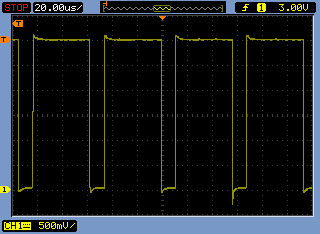
\includegraphics[width=0.45\textwidth]{img/pwm1.png}}
	\makebox[0.45\textwidth]{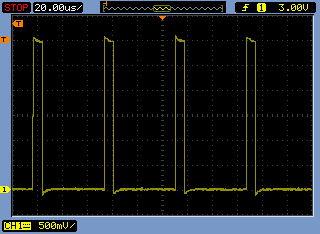
\includegraphics[width=0.45\textwidth]{img/pwm2.png}}
	\caption{Změřené PWM výstupní signály}
	\label{fig:pwm}
\end{figure}

\section{Real-time Server}
Server je naprogramovaný v JavaScriptu s využitím Sails.js \index{Sails} frameworku \cite{sails}. Tento framework staví nad Express frameworkem, který staví nad Node.js. Node.js je platforma postavená nad V8 \cite{v8}, tedy JavaScriptovém jádře napsaném v C++. Toto jádro je například součástí prohlížeče Chrome. \index{V8} Kromě toho, že toto jádro dosahuje vysokého výkonu při zpracování JS, otevírá také zajímavé možnosti, jak přistupovat k programu. Konkrétně nabízí například event-driven chování, nebo neblokující I/O model. Toto chování vychází z JavaScriptu jako takového. To může být svým způsobem zároveň nevýhoda. JavaScript se totiž chová (v běžných implementacích) jako jednovláknový asynchronní program. To sice umožňuje vytvářet zajímavé programové struktury, zároveň je však limitující jedno vlákno. Je proto lepší spustit odděleně webovou aplikaci a část zpracovávající příchozí signály. Každá tato část lze pak v případě potřeby spustit v clusteru \cite{cluster}. Adresářová struktura je zobrazena níže. Opět jsou znázorněny jen důležité části. Tato struktura odpovídá běžné struktuře Sails.js \cite{sails} aplikace s EJS šablonovacím systémem.

\begin{figure}[H]
\dirtree{%
.1 /. 
.2 redis\DTcomment{Redis server pro Windows}. 
.2 server\DTcomment{soubory real-time serveru}. 
.3 .tmp\DTcomment{dočasné soubory aplikace}. 
.3 api\DTcomment{modely a kontroléry aplikace}. 
.4 controllers\DTcomment{kontroléry}. 
.4 hooks\DTcomment{eventy}. 
.4 models\DTcomment{modely}. 
.4 policies\DTcomment{skripty upravující chování aplikace}. 
.4 responses\DTcomment{HTTP odpovědi serveru}. 
.4 services\DTcomment{služby}. 
.3 assets\DTcomment{obrázky, skripty a styly}. 
.3 config\DTcomment{konfigurační soubory}. 
.3 node\_modules\DTcomment{nainstalované knihovny přes NPM}. 
.3 tasks\DTcomment{úkoly pro Grunt}. 
.3 views\DTcomment{šablony aplikace}. 
.4 Device\DTcomment{šablony pro DeviceController.js}. 
.4 Documentation\DTcomment{šablony pro dokumentaci}. 
.4 Homepage\DTcomment{šablony pro HomepageController.js}. 
.4 layout.ejs\DTcomment{layout pro šablony aplikace}. 
.4 .... 
.3 app.js\DTcomment{script automatický start serveru}. 
.3 Gruntfile.js\DTcomment{startovací skript pro Grunt}. 
.3 package.json\DTcomment{JSON soubor pro NPM}. 
.3 .... 
.2 start.bat\DTcomment{startovací script}. 
}
\end{figure}

Celý server lze nastartovat souborem \texttt{start.bat}, jehož obsah je zná\-zor\-něn níže.

\begin{minted}[linenos,breaklines]{bat}
@echo off

cd .\redis\bin\release\redis-2.8.17
start redis-server.exe

cd .\..\..\..\..\server
sails lift

exit
\end{minted}

Je tedy zřejmé, že je nutné nastartovat Redis databázi a následně samotnou aplikaci pomocí příkazu \texttt{sails lift}. Při prvním spuštění je také nutné doinstalovat závislosti pomocí NPM. Pokud by bylo nežádoucí spouštět aplikaci pomocí Sails.js, je možné použít klasický Node.js (\texttt{node app.js}). samotný framework tedy neomezuje aplikaci a tu je tak možné přenést do jiného prostředí jako je například Heroku \cite{heroku}, nebo využít podpůrné nástroje jako je Forever \cite{forever} (\texttt{forever start app.js}), který zajistí, že program poběží nepřetržitě tzn. i po fatální chybě.

Celá aplikace je rozdělena na několik částí. První jsou šablony jednotlivých stránek. Tyto šablony využívají šablonovací systém EJS. Tyto šablony mají asi nejpřijatelnější zápis ze všech ostatních:

\begin{minted}[linenos,breaklines]{text}
<h1><%= variable %></h1>
<ul>
  <% for(var i = 0; i < xarray.length; i++) { %>
    <li><%= xarray[i] %></li>
  <% } %>
</ul>
<%= img_tag('images/picture.png') %>
\end{minted}

Do této šablony se předávají data z controlleru (zjednodušeně):

\begin{minted}[linenos,breaklines]{js}
module.exports = {

  index: function (request, response) {
    RedisService.smembers('devices', function (err, result) {
      res.view({
        xarray: result,
        varibale: 'example'
      });
    });
  }

};
\end{minted}

Při psaní takových programů je nutné mít na paměti, že se kód může (a bude) vykonávat asynchronně. Proto je nutné všechny synchronní operace provádět pomocí callbacků, nebo například přes návrhový vzor promise. \index{Promise} Rozdíly mezi těmito přístupy jsou popsány níže. Návrhový vzor promise ale není tolik rozšířený, takže se všude v tomto programu používá první přístup. Základní rozdíl je v tom, že běžné je v Node.js funkce kvůli synchronnímu chování zanořovat:

\begin{minted}[linenos,breaklines]{js}
step1(function (value1) {
  step2(value1, function(value2) {
    step3(value2, function(value3) {
      step4(value3, function(value4) {
        console.log(value4);
      });
    });
  });
});
\end{minted}

Zatímco s promise návrhovým vzorem zanořování není nutné:

\begin{minted}[linenos,breaklines]{js}
Q.fcall(promisedStep1)
.then(promisedStep2)
.then(promisedStep3)
.then(promisedStep4)
.then(function (value4) {
  console.log(value4);
})
.catch(function (error) {
  console.error(value4);
})
.done();
\end{minted}

Je možné použít knihovnu Q \cite{q} ze které jsou tyto příklady přebrány. Toto chování by mělo být v pozdějších verzích JavaScriptu k dispozici bez potřeby knihoven třetích stran. Vzhledem k tomu, že použití callbacků má celou řadu nevýhod, návrhový vzor promise se stává velmi populárním a postupně na něj přecházejí všechny velké knihovny.

Samotná aplikace využívá následující tabulky v Redis databázi, kde \texttt{xxx} je unikátní identifikátor zařízení: \index{Redis}

\begin{itemize}
\itemsep0em
\item \texttt{devices} (set) - obsahuje unikátní identifikátory připojených zařízení
\item \texttt{device:xxx} (hash) - informace o konkrétním zařízení:
	\begin{itemize}
	\itemsep0em
		\item \texttt{ip} - IP adresa zařízení
		\item \texttt{port} - TCP port
		\item \texttt{active} - logická hodnota určující, jestli je zařízení aktivní
		\item \texttt{last\_ping} - čas posledního ohlášení
		\item \texttt{msg\_count} - počet vyměněných zpráv se serverem
		\item \texttt{udp\_port} - UDP port
		\item \texttt{function} - zvolená funkce pro přepočet hodnot
	\end{itemize}
\item \texttt{xxx:data} (list) - historie přijatých dat ze zařízení (posledních 1000 hodnot)
\item \texttt{xxx:table} (hash) - vypočtená převodní tabulka
\item \texttt{connection:xxx} (set) - tabulka uchovávající relace
\end{itemize}

Dále je pak k dispozici hodnota \texttt{msg\_count}, která udržuje počet vy\-mě\-ně\-ných zpráv s jakýmkoliv zařízením připojeným do sítě.

\subsection{Komunikace s koncentrátory}
Server komunikuje s koncentrátory hlavně pomocí UDP. Celá logika je u\-mís\-tě\-na v souboru \texttt{api/hooks/UDP/index.js}, kde je také vyřešené odeslání UDP datagramů. Tento script je ve formě tzv. hooku. Volně by se tento termín dal přeložit jako \uv{hák}, což jej přesně vystihuje. Tento kód se totiž navěsí na okamžik spouštění celé aplikace, ještě před nastartováním webového serveru. Je zde použit callback přístup, nikoliv návrhový vzor promise. Z důvodu složitosti zde neuvádím žádné ukázky kódu, za zmínku však stojí jedna zajímavá vlastnost, která je společná pro server i koncentrátory. Ve skutečnosti totiž neodesílají data pořád, ale pouze pokud je to potřeba, tzn. pokud se nová informace liší od předchozí. Tímto se zásadně sníží počet přenášených datagramů a je možné zvýšit rychlost cyklu. Je potřeba myslet na to, že nikdy nenastane dlouhá doba, kdy by se koncentrátor úplně odmlčel. Koncentrátor se totiž pravidelně ohlašuje serveru, čímž říká, že je stále aktivní a správně funguje. Právě na tomto místě pak dochází k využívání převodních tabulek, které jsou podrobně popsány v další kapitole. Podobná logika je k nalezení i v souboru \texttt{api/hooks/TCP/index.js} pro TCP. V souboru \texttt{api/hooks/routine.js} dochází k vyhodnocování aktivity připojených zařízení na základě posledního ohlášení.

\subsection{Webový server}
Kromě real-time serveru existuje také webový server, který zabírá ve složce \texttt{server} nejvíce místa. Jednou z hlavních složek tohoto serveru, kromě již zmíněných šablon a kontrolérů, je část obsluhující websocket. Ta je k nalezení v souboru \texttt{api/hooks/websocket.js}. V tomto projektu je použita část frameworku Sails.js \cite{sails}, která websockety obsluhuje, fakticky však pouze zabaluje knihovnu Socket.IO \cite{socket}. Následuje zjednodušená ukázka použití této knihovny a to včetně zabalení kódu tak, aby se choval jako hook a spustil se při startu aplikace:

\begin{minted}[linenos,breaklines]{js}
module.exports = function WebsocketHook(sails) {
  return {
    start: function () {
      sails.io.on('connection', function (socket) {
        RedisService.smembers('devices', function (err, result) {
          socket.emit('devices', result);
        });
      });
      sails.log('Starting WEBSOCKET server...');
    },
    initialize: function (cb) {
      var hook = this;
      hook.start();
      return cb();
    }
  }
};
\end{minted}

Sails.js při startování serveru zavolá metodu \texttt{initialize}. Ta následně spustí požadovaný kód, v tomto případě odesílá při připojení klienta informace o všech zařízeních, které jsou k dispozici. Právě v této části serveru dochází k další zajímavé vlastnosti celého systému. Momentálně se totiž všechny informace v síti posílají jako desítková celá čísla v rozsahu 0-1023. Tzn. že například výstupem z ADC je jedna z hodnot v tomto rozsahu. Výhodné je to, že je možné jednoduše tuto informaci na serveru upravovat. Jednou z úprav jsou například nelinearity. Další je však jednoduchý klouzavý průměr (SMA). Protože příchozí data se nepatrně mění v jednotkovém rozsahu například vlivem nečistot potenciometru, je nutné tuto informaci vyhladit. Toto vyhlazení je pouze z estetických důvodů, protože vzhledem k tomu, jak je celý systém rychlý, toto přeskakování se dostane i do uživatelského rozhraní a to nepůsobí dobře. Konkrétně se vypočítává SMA z posledních pěti hodnot:

\begin{equation}
	SMA = \dfrac{X_t + X_{t-1} + X_{t-2} + X_{t-3} + X_{t-4}}{5}
	\label{eq:sma}
\end{equation}

Klouzavý průměr se tedy používá pouze při výstupu do webové aplikace. Jinak funguje celá síť s takovou informací, jaká opustila koncentrátor. Je nutné myslet na to, že klouzavý průměr sice vyhlazuje výkyvy v průběhu, zároveň však celý průběh zpomaluje. Toto zpomalení je pak větší se zvět\-šu\-jí\-cím se počtem vzorků, které se do SMA zahrnují.

Velkou výhodou je fakt, že je celý systém možné ovládat z webové aplikace. Tu je možné otevřít téměř na jakémkoliv zařízení, které je připojené k internetu. Celou aplikaci je však ještě možné zabalit do nativní mobilní aplikace například pomocí Apache Cordova \cite{cordova}, takže lze na jakékoliv mobilní zařízení nainstalovat. \index{Apache Cordova} Nejedná se sice o nejlepší způsob jak takovou aplikaci postavit, je to však mnohem rychlejší a levnější cesta. Některé frameworky, jako například Meteor umožňují tyto aplikaci vystavit již v základu pomocí dvou příkazů \cite{meteor}. Tento framework však nebyl zvolen, protože nemá dobrou integraci Redis \cite{redis} databáze a hodí se na jiné aplikace, kde je možné využít principu \uv{latency compensation}, \index{Latency compensation} tedy kompenzace času spotřebovaného pro komunikaci mezi serverem a prohlížečem. Toho je docíleno tak, že se programové metody umístí jak na server, tak na klientskou stranu. Následně při požadavku se metody zavolají na serveru, ale framework na straně klienta nečeká a provede simulaci dané operace i v prohlížeči. Tak je možné některé operace zpracovat ještě před odpovědí serveru. Pokud se výsledek operace ze serveru shoduje s výsledkem na straně klienta, vše je v pořádku. V opačném případě se provedené změny vrátí zpět a prohlížeč skutečně zrcadlí stav serveru. V případě úspěšné operace se tedy aplikace chová velmi rychle, jinak může docházet ke zvláštnímu chování uživatelského prostředí. Takto samozřejmě není možné provádět operace čekající na výsledek z databáze.